\let\negmpace\undefined
\let\negthickspace\undefined
\documentclass[journal]{IEEEtran}
\usepackage[a5paper, margin=10mm, onecolumn]{geometry}
%\usepackage{lmodern} % Ensure lmodern is loaded for pdflatex
\usepackage{tfrupee} % Include tfrupee package
\setlength{\headheight}{1cm} % Set the height of the header box
\setlength{\headsep}{0mm}     % Set the distance between the header box and the top of the text
\usepackage{xparse}
\usepackage{gvv-book}
\usepackage{gvv}
\usepackage{cite}
\usepackage{amsmath,amssymb,amsfonts,amsthm}
\usepackage{algorithmic}
\usepackage{graphicx}
\usepackage{textcomp}
\usepackage{xcolor}
\usepackage{txfonts}
\usepackage{listings}
\usepackage{enumitem}
\usepackage{mathtools}
\usepackage{gensymb}
\usepackage{comment}
\usepackage[breaklinks=true]{hyperref}
\usepackage{tkz-euclide} 
\usepackage{listings}
% \usepackage{gvv}                                        
\def\inputGnumericTable{}                                 
\usepackage[latin1]{inputenc}                                
\usepackage{color}                                            
\usepackage{array}                                            
\usepackage{longtable}                                       
\usepackage{calc}                                             
\usepackage{multirow}                                         
\usepackage{hhline}                                           
\usepackage{ifthen}                                           
\usepackage{lscape}
\renewcommand{\thefigure}{\theenumi}
\renewcommand{\thetable}{\theenumi}
\setlength{\intextsep}{10pt} % Space between text and floats
\numberwithin{equation}{enumi}
\numberwithin{figure}{enumi}
\renewcommand{\thetable}{\theenumi}
\begin{document}
\bibliographystyle{IEEEtran}
\title{Question-9.4.9}
\author{EE24BTECH11038 - MALAKALA BALA SUBRAHMANYA ARAVIND}
% \maketitle
% \newpage
% \bigskip
{\let\newpage\relax\maketitle}
\textbf{Question}:
$\frac{dy}{dx}$ = $\sin^{-1}{x}$\\


\solution \\
Integrate on both sides
\begin{align}
    \int dy=\int \sin^{-1}{x}\,\,dx
\end{align}
Using integration by parts
\begin{align}
    y&=x\sin^{-1}{x}-\int \frac{x}{\sqrt{1-x^{2}}}\,\,dx\\   
    t&=\sqrt{1-x^2}\\
    dt&=\frac{-2x}{\sqrt{1-x^2}}\,\,dx\\
    y&=x\sin^{-1}x+\int \frac{dt}{2\sqrt{t}}\\
    y&=x\sin^{-1}{x}+\sqrt{t}+c
\end{align}
substituting value of t gives
\begin{align}
    y&=x\sin^{-1}{x}+\sqrt{1-x^2}+c
\end{align}
Let the intital conditions be $X_{0}=0,Y_{0}=1$
\begin{align}
    1&=0+1+c\\
    c&=0
\end{align}
Final equation of the curve
\begin{align}
    Y&=x\sin^{-1}{x}+\sqrt{1-x^2}
\end{align}
Now let us  this computationally from the definition of $\frac{dy}{dx}$ 
\begin{align}
    Y_{n+1}=Y_n+\frac{dy}{dx}.h
\end{align}
From the differential equation
\begin{align}
    \frac{dy}{dx}=\frac{y_n-x_n}{y_n+x_n}.h\\
    y_{n+1}=y_n+\brak{\frac{y_n-x_n}{y_n+x_n}}.h
\end{align}
BY taking $x_1$=0 and $y_1$=1 and h=0.01 going till x=1 by iterating through the loop and finding $y_2,y_3,y_4,\cdots$ and plotting the graph. we can verify the function we got by solving the differential equation mathematically
\begin{figure}[!ht]
    \centering
    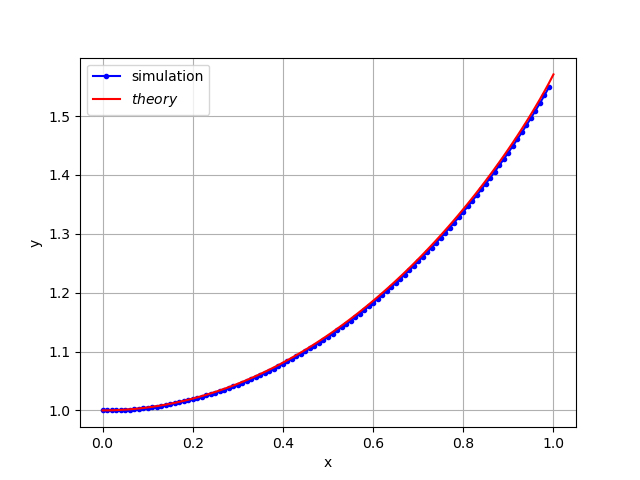
\includegraphics[width=\columnwidth]{figs/Figure_1.png}
    \caption{}
\end{figure}
\end{document}
